\documentclass[twoside]{book}

% Packages required by doxygen
\usepackage{fixltx2e}
\usepackage{calc}
\usepackage{doxygen}
\usepackage[export]{adjustbox} % also loads graphicx
\usepackage{graphicx}
\usepackage[utf8]{inputenc}
\usepackage{makeidx}
\usepackage{multicol}
\usepackage{multirow}
\PassOptionsToPackage{warn}{textcomp}
\usepackage{textcomp}
\usepackage[nointegrals]{wasysym}
\usepackage[table]{xcolor}

% Font selection
\usepackage[T1]{fontenc}
\usepackage[scaled=.90]{helvet}
\usepackage{courier}
\usepackage{amssymb}
\usepackage{sectsty}
\renewcommand{\familydefault}{\sfdefault}
\allsectionsfont{%
  \fontseries{bc}\selectfont%
  \color{darkgray}%
}
\renewcommand{\DoxyLabelFont}{%
  \fontseries{bc}\selectfont%
  \color{darkgray}%
}
\newcommand{\+}{\discretionary{\mbox{\scriptsize$\hookleftarrow$}}{}{}}

% Page & text layout
\usepackage{geometry}
\geometry{%
  a4paper,%
  top=2.5cm,%
  bottom=2.5cm,%
  left=2.5cm,%
  right=2.5cm%
}
\tolerance=750
\hfuzz=15pt
\hbadness=750
\setlength{\emergencystretch}{15pt}
\setlength{\parindent}{0cm}
\setlength{\parskip}{3ex plus 2ex minus 2ex}
\makeatletter
\renewcommand{\paragraph}{%
  \@startsection{paragraph}{4}{0ex}{-1.0ex}{1.0ex}{%
    \normalfont\normalsize\bfseries\SS@parafont%
  }%
}
\renewcommand{\subparagraph}{%
  \@startsection{subparagraph}{5}{0ex}{-1.0ex}{1.0ex}{%
    \normalfont\normalsize\bfseries\SS@subparafont%
  }%
}
\makeatother

% Headers & footers
\usepackage{fancyhdr}
\pagestyle{fancyplain}
\fancyhead[LE]{\fancyplain{}{\bfseries\thepage}}
\fancyhead[CE]{\fancyplain{}{}}
\fancyhead[RE]{\fancyplain{}{\bfseries\leftmark}}
\fancyhead[LO]{\fancyplain{}{\bfseries\rightmark}}
\fancyhead[CO]{\fancyplain{}{}}
\fancyhead[RO]{\fancyplain{}{\bfseries\thepage}}
\fancyfoot[LE]{\fancyplain{}{}}
\fancyfoot[CE]{\fancyplain{}{}}
\fancyfoot[RE]{\fancyplain{}{\bfseries\scriptsize Generated by Doxygen }}
\fancyfoot[LO]{\fancyplain{}{\bfseries\scriptsize Generated by Doxygen }}
\fancyfoot[CO]{\fancyplain{}{}}
\fancyfoot[RO]{\fancyplain{}{}}
\renewcommand{\footrulewidth}{0.4pt}
\renewcommand{\chaptermark}[1]{%
  \markboth{#1}{}%
}
\renewcommand{\sectionmark}[1]{%
  \markright{\thesection\ #1}%
}

% Indices & bibliography
\usepackage{natbib}
\usepackage[titles]{tocloft}
\setcounter{tocdepth}{3}
\setcounter{secnumdepth}{5}
\makeindex

% Hyperlinks (required, but should be loaded last)
\usepackage{ifpdf}
\ifpdf
  \usepackage[pdftex,pagebackref=true]{hyperref}
\else
  \usepackage[ps2pdf,pagebackref=true]{hyperref}
\fi
\hypersetup{%
  colorlinks=true,%
  linkcolor=blue,%
  citecolor=blue,%
  unicode%
}

% Custom commands
\newcommand{\clearemptydoublepage}{%
  \newpage{\pagestyle{empty}\cleardoublepage}%
}

\usepackage{caption}
\captionsetup{labelsep=space,justification=centering,font={bf},singlelinecheck=off,skip=4pt,position=top}

%===== C O N T E N T S =====

\begin{document}

% Titlepage & ToC
\hypersetup{pageanchor=false,
             bookmarksnumbered=true,
             pdfencoding=unicode
            }
\pagenumbering{alph}
\begin{titlepage}
\vspace*{7cm}
\begin{center}%
{\Large Operaciones Pila }\\
\vspace*{1cm}
{\large Generated by Doxygen 1.8.13}\\
\end{center}
\end{titlepage}
\clearemptydoublepage
\pagenumbering{roman}
\tableofcontents
\clearemptydoublepage
\pagenumbering{arabic}
\hypersetup{pageanchor=true}

%--- Begin generated contents ---
\chapter{Namespace Index}
\section{Namespace List}
Here is a list of all documented namespaces with brief descriptions\+:\begin{DoxyCompactList}
\item\contentsline{section}{\hyperlink{namespace_operaciones_pila}{Operaciones\+Pila} }{\pageref{namespace_operaciones_pila}}{}
\end{DoxyCompactList}

\chapter{Hierarchical Index}
\section{Class Hierarchy}
This inheritance list is sorted roughly, but not completely, alphabetically\+:\begin{DoxyCompactList}
\item Application\begin{DoxyCompactList}
\item \contentsline{section}{Operaciones\+Pila.\+App}{\pageref{class_operaciones_pila_1_1_app}}{}
\end{DoxyCompactList}
\item \contentsline{section}{Operaciones\+Pila.\+Array\+Stack$<$ T $>$}{\pageref{class_operaciones_pila_1_1_array_stack}}{}
\item \contentsline{section}{Operaciones\+Pila.\+Array\+Stack$<$ string $>$}{\pageref{class_operaciones_pila_1_1_array_stack}}{}
\item Exception\begin{DoxyCompactList}
\item \contentsline{section}{Operaciones\+Pila.\+Empty\+Stack\+Exception}{\pageref{class_operaciones_pila_1_1_empty_stack_exception}}{}
\item \contentsline{section}{Operaciones\+Pila.\+Full\+Stack\+Exception}{\pageref{class_operaciones_pila_1_1_full_stack_exception}}{}
\end{DoxyCompactList}
\item Window\begin{DoxyCompactList}
\item \contentsline{section}{Operaciones\+Pila.\+Main\+Window}{\pageref{class_operaciones_pila_1_1_main_window}}{}
\end{DoxyCompactList}
\end{DoxyCompactList}

\chapter{Class Index}
\section{Class List}
Here are the classes, structs, unions and interfaces with brief descriptions\+:\begin{DoxyCompactList}
\item\contentsline{section}{\hyperlink{class_operaciones_pila_1_1_app}{Operaciones\+Pila.\+App} \\*Interaction logic for App.\+xaml }{\pageref{class_operaciones_pila_1_1_app}}{}
\item\contentsline{section}{\hyperlink{class_operaciones_pila_1_1_array_stack}{Operaciones\+Pila.\+Array\+Stack$<$ T $>$} }{\pageref{class_operaciones_pila_1_1_array_stack}}{}
\item\contentsline{section}{\hyperlink{class_operaciones_pila_1_1_empty_stack_exception}{Operaciones\+Pila.\+Empty\+Stack\+Exception} }{\pageref{class_operaciones_pila_1_1_empty_stack_exception}}{}
\item\contentsline{section}{\hyperlink{class_operaciones_pila_1_1_full_stack_exception}{Operaciones\+Pila.\+Full\+Stack\+Exception} }{\pageref{class_operaciones_pila_1_1_full_stack_exception}}{}
\item\contentsline{section}{\hyperlink{class_operaciones_pila_1_1_main_window}{Operaciones\+Pila.\+Main\+Window} \\*Interaction logic for Main\+Window.\+xaml }{\pageref{class_operaciones_pila_1_1_main_window}}{}
\end{DoxyCompactList}

\chapter{Namespace Documentation}
\hypertarget{namespace_operaciones_pila}{}\section{Operaciones\+Pila Namespace Reference}
\label{namespace_operaciones_pila}\index{Operaciones\+Pila@{Operaciones\+Pila}}
\subsection*{Classes}
\begin{DoxyCompactItemize}
\item 
class \hyperlink{class_operaciones_pila_1_1_app}{App}
\begin{DoxyCompactList}\small\item\em Interaction logic for App.\+xaml \end{DoxyCompactList}\item 
class \hyperlink{class_operaciones_pila_1_1_array_stack}{Array\+Stack}
\item 
class \hyperlink{class_operaciones_pila_1_1_empty_stack_exception}{Empty\+Stack\+Exception}
\item 
class \hyperlink{class_operaciones_pila_1_1_full_stack_exception}{Full\+Stack\+Exception}
\item 
class \hyperlink{class_operaciones_pila_1_1_main_window}{Main\+Window}
\begin{DoxyCompactList}\small\item\em Interaction logic for Main\+Window.\+xaml \end{DoxyCompactList}\end{DoxyCompactItemize}

\chapter{Class Documentation}
\hypertarget{class_operaciones_pila_1_1_app}{}\section{Operaciones\+Pila.\+App Class Reference}
\label{class_operaciones_pila_1_1_app}\index{Operaciones\+Pila.\+App@{Operaciones\+Pila.\+App}}


Interaction logic for App.\+xaml  


Inheritance diagram for Operaciones\+Pila.\+App\+:\begin{figure}[H]
\begin{center}
\leavevmode
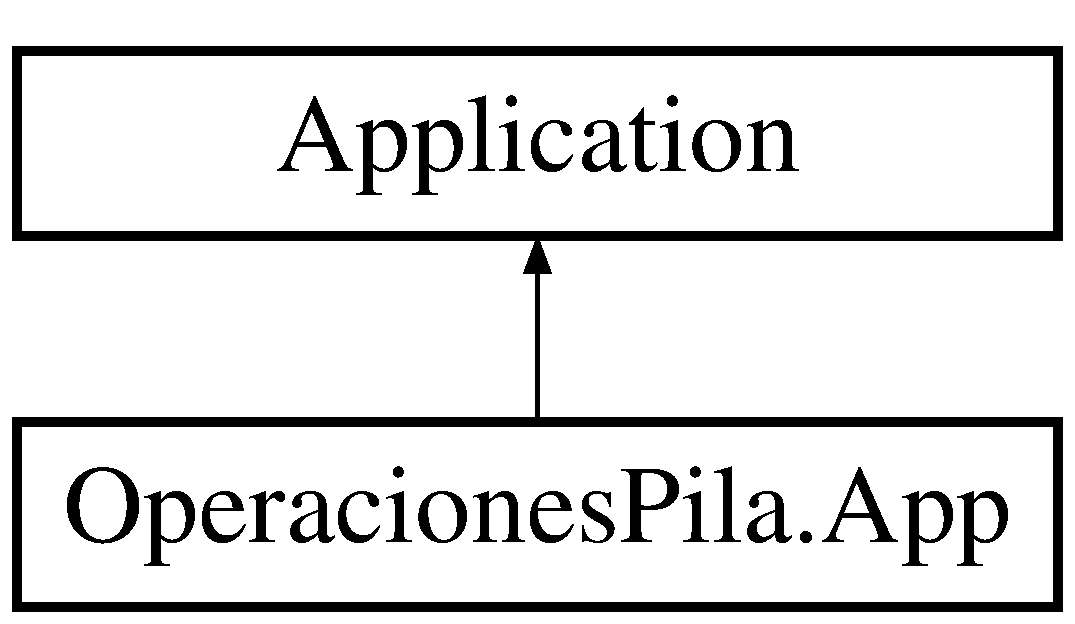
\includegraphics[height=2.000000cm]{class_operaciones_pila_1_1_app}
\end{center}
\end{figure}


\subsection{Detailed Description}
Interaction logic for App.\+xaml 



The documentation for this class was generated from the following file\+:\begin{DoxyCompactItemize}
\item 
D\+:/\+U\+N\+I/3er Semestre/\+Estructuras/\+S (3)/\+Operaciones\+Pila/\+Operaciones\+Pila/App.\+xaml.\+cs\end{DoxyCompactItemize}

\hypertarget{class_operaciones_pila_1_1_array_stack}{}\section{Operaciones\+Pila.\+Array\+Stack$<$ T $>$ Class Template Reference}
\label{class_operaciones_pila_1_1_array_stack}\index{Operaciones\+Pila.\+Array\+Stack$<$ T $>$@{Operaciones\+Pila.\+Array\+Stack$<$ T $>$}}
\subsection*{Public Member Functions}
\begin{DoxyCompactItemize}
\item 
\hyperlink{class_operaciones_pila_1_1_array_stack_a71fa2281672474bbef92556bf944a176}{Array\+Stack} (int max\+Size)
\begin{DoxyCompactList}\small\item\em Constructor. \end{DoxyCompactList}\item 
int \hyperlink{class_operaciones_pila_1_1_array_stack_aef6d20149157d51dafe5c7a0c70275a9}{Size} ()
\begin{DoxyCompactList}\small\item\em Entrada\+: nada Salidas\+: Devuelve la cantidad de elementos en la pila. Poscondicion\+: Los datos permanecen sin cambio. \end{DoxyCompactList}\item 
void \hyperlink{class_operaciones_pila_1_1_array_stack_a24832d21024200fba53690fe399277e6}{Push} (T item)
\begin{DoxyCompactList}\small\item\em Entradas\+: el elemento de tipo T que se desea ingresar a la pila Salidas\+: Lanza una \hyperlink{class_operaciones_pila_1_1_full_stack_exception}{Full\+Stack\+Exception} si la pila esta llena. Poscondicion\+: Si la pila no esta llena, se agrega el elemento al top de la pila. \end{DoxyCompactList}\item 
T \hyperlink{class_operaciones_pila_1_1_array_stack_a077d65f90d9b421a881dab181e136147}{Pop} ()
\begin{DoxyCompactList}\small\item\em Entradas\+: ninguna. Salidas\+: Si la pila esta vacia, lanza una \hyperlink{class_operaciones_pila_1_1_empty_stack_exception}{Empty\+Stack\+Exception}. Si no esta vacia, remueve y devuelve el elemento que esta en la posicion top de la pila. Poscondicion\+: Si la pila no esta vacia, se remueve el elemento top de la pila. \end{DoxyCompactList}\item 
T \hyperlink{class_operaciones_pila_1_1_array_stack_ac0b80f6ed3ef56c01e9fd4c847504444}{Peek} ()
\begin{DoxyCompactList}\small\item\em Entradas\+:ninguna. Salidas\+: Si la pila esta vacia, lanza una \hyperlink{class_operaciones_pila_1_1_empty_stack_exception}{Empty\+Stack\+Exception}. Si no esta vacia, devuelve el elemento en la posicion top de la pila. Poscondicion\+: Los datos permanecen sin cambio. \end{DoxyCompactList}\end{DoxyCompactItemize}
\subsection*{Private Attributes}
\begin{DoxyCompactItemize}
\item 
\mbox{\Hypertarget{class_operaciones_pila_1_1_array_stack_af3e83c01e1e9acb877368f2c84f7b2af}\label{class_operaciones_pila_1_1_array_stack_af3e83c01e1e9acb877368f2c84f7b2af}} 
T \mbox{[}$\,$\mbox{]} {\bfseries stack}
\item 
\mbox{\Hypertarget{class_operaciones_pila_1_1_array_stack_a2fdd9c8be1b81c13ca35da135cbec7be}\label{class_operaciones_pila_1_1_array_stack_a2fdd9c8be1b81c13ca35da135cbec7be}} 
int {\bfseries top}
\item 
\mbox{\Hypertarget{class_operaciones_pila_1_1_array_stack_ae90b2997e9685d9de9300746947b6b96}\label{class_operaciones_pila_1_1_array_stack_ae90b2997e9685d9de9300746947b6b96}} 
int {\bfseries max\+Size}
\end{DoxyCompactItemize}


\subsection{Constructor \& Destructor Documentation}
\mbox{\Hypertarget{class_operaciones_pila_1_1_array_stack_a71fa2281672474bbef92556bf944a176}\label{class_operaciones_pila_1_1_array_stack_a71fa2281672474bbef92556bf944a176}} 
\index{Operaciones\+Pila\+::\+Array\+Stack@{Operaciones\+Pila\+::\+Array\+Stack}!Array\+Stack@{Array\+Stack}}
\index{Array\+Stack@{Array\+Stack}!Operaciones\+Pila\+::\+Array\+Stack@{Operaciones\+Pila\+::\+Array\+Stack}}
\subsubsection{\texorpdfstring{Array\+Stack()}{ArrayStack()}}
{\footnotesize\ttfamily \hyperlink{class_operaciones_pila_1_1_array_stack}{Operaciones\+Pila.\+Array\+Stack}$<$ T $>$.\hyperlink{class_operaciones_pila_1_1_array_stack}{Array\+Stack} (\begin{DoxyParamCaption}\item[{int}]{max\+Size }\end{DoxyParamCaption})\hspace{0.3cm}{\ttfamily [inline]}}



Constructor. 


\begin{DoxyParams}{Parameters}
{\em max\+Size} & El tamaño de la pila.\\
\hline
\end{DoxyParams}


\subsection{Member Function Documentation}
\mbox{\Hypertarget{class_operaciones_pila_1_1_array_stack_ac0b80f6ed3ef56c01e9fd4c847504444}\label{class_operaciones_pila_1_1_array_stack_ac0b80f6ed3ef56c01e9fd4c847504444}} 
\index{Operaciones\+Pila\+::\+Array\+Stack@{Operaciones\+Pila\+::\+Array\+Stack}!Peek@{Peek}}
\index{Peek@{Peek}!Operaciones\+Pila\+::\+Array\+Stack@{Operaciones\+Pila\+::\+Array\+Stack}}
\subsubsection{\texorpdfstring{Peek()}{Peek()}}
{\footnotesize\ttfamily T \hyperlink{class_operaciones_pila_1_1_array_stack}{Operaciones\+Pila.\+Array\+Stack}$<$ T $>$.Peek (\begin{DoxyParamCaption}{ }\end{DoxyParamCaption})\hspace{0.3cm}{\ttfamily [inline]}}



Entradas\+:ninguna. Salidas\+: Si la pila esta vacia, lanza una \hyperlink{class_operaciones_pila_1_1_empty_stack_exception}{Empty\+Stack\+Exception}. Si no esta vacia, devuelve el elemento en la posicion top de la pila. Poscondicion\+: Los datos permanecen sin cambio. 

\begin{DoxyReturn}{Returns}

\end{DoxyReturn}
\mbox{\Hypertarget{class_operaciones_pila_1_1_array_stack_a077d65f90d9b421a881dab181e136147}\label{class_operaciones_pila_1_1_array_stack_a077d65f90d9b421a881dab181e136147}} 
\index{Operaciones\+Pila\+::\+Array\+Stack@{Operaciones\+Pila\+::\+Array\+Stack}!Pop@{Pop}}
\index{Pop@{Pop}!Operaciones\+Pila\+::\+Array\+Stack@{Operaciones\+Pila\+::\+Array\+Stack}}
\subsubsection{\texorpdfstring{Pop()}{Pop()}}
{\footnotesize\ttfamily T \hyperlink{class_operaciones_pila_1_1_array_stack}{Operaciones\+Pila.\+Array\+Stack}$<$ T $>$.Pop (\begin{DoxyParamCaption}{ }\end{DoxyParamCaption})\hspace{0.3cm}{\ttfamily [inline]}}



Entradas\+: ninguna. Salidas\+: Si la pila esta vacia, lanza una \hyperlink{class_operaciones_pila_1_1_empty_stack_exception}{Empty\+Stack\+Exception}. Si no esta vacia, remueve y devuelve el elemento que esta en la posicion top de la pila. Poscondicion\+: Si la pila no esta vacia, se remueve el elemento top de la pila. 

\begin{DoxyReturn}{Returns}

\end{DoxyReturn}
\mbox{\Hypertarget{class_operaciones_pila_1_1_array_stack_a24832d21024200fba53690fe399277e6}\label{class_operaciones_pila_1_1_array_stack_a24832d21024200fba53690fe399277e6}} 
\index{Operaciones\+Pila\+::\+Array\+Stack@{Operaciones\+Pila\+::\+Array\+Stack}!Push@{Push}}
\index{Push@{Push}!Operaciones\+Pila\+::\+Array\+Stack@{Operaciones\+Pila\+::\+Array\+Stack}}
\subsubsection{\texorpdfstring{Push()}{Push()}}
{\footnotesize\ttfamily void \hyperlink{class_operaciones_pila_1_1_array_stack}{Operaciones\+Pila.\+Array\+Stack}$<$ T $>$.Push (\begin{DoxyParamCaption}\item[{T}]{item }\end{DoxyParamCaption})\hspace{0.3cm}{\ttfamily [inline]}}



Entradas\+: el elemento de tipo T que se desea ingresar a la pila Salidas\+: Lanza una \hyperlink{class_operaciones_pila_1_1_full_stack_exception}{Full\+Stack\+Exception} si la pila esta llena. Poscondicion\+: Si la pila no esta llena, se agrega el elemento al top de la pila. 


\begin{DoxyParams}{Parameters}
{\em item} & \\
\hline
\end{DoxyParams}
\mbox{\Hypertarget{class_operaciones_pila_1_1_array_stack_aef6d20149157d51dafe5c7a0c70275a9}\label{class_operaciones_pila_1_1_array_stack_aef6d20149157d51dafe5c7a0c70275a9}} 
\index{Operaciones\+Pila\+::\+Array\+Stack@{Operaciones\+Pila\+::\+Array\+Stack}!Size@{Size}}
\index{Size@{Size}!Operaciones\+Pila\+::\+Array\+Stack@{Operaciones\+Pila\+::\+Array\+Stack}}
\subsubsection{\texorpdfstring{Size()}{Size()}}
{\footnotesize\ttfamily int \hyperlink{class_operaciones_pila_1_1_array_stack}{Operaciones\+Pila.\+Array\+Stack}$<$ T $>$.Size (\begin{DoxyParamCaption}{ }\end{DoxyParamCaption})\hspace{0.3cm}{\ttfamily [inline]}}



Entrada\+: nada Salidas\+: Devuelve la cantidad de elementos en la pila. Poscondicion\+: Los datos permanecen sin cambio. 

\begin{DoxyReturn}{Returns}

\end{DoxyReturn}


The documentation for this class was generated from the following file\+:\begin{DoxyCompactItemize}
\item 
D\+:/\+U\+N\+I/3er Semestre/\+Estructuras/\+S (3)/\+Operaciones\+Pila/\+Operaciones\+Pila/Array\+Stack.\+cs\end{DoxyCompactItemize}

\hypertarget{class_operaciones_pila_1_1_empty_stack_exception}{}\section{Operaciones\+Pila.\+Empty\+Stack\+Exception Class Reference}
\label{class_operaciones_pila_1_1_empty_stack_exception}\index{Operaciones\+Pila.\+Empty\+Stack\+Exception@{Operaciones\+Pila.\+Empty\+Stack\+Exception}}
Inheritance diagram for Operaciones\+Pila.\+Empty\+Stack\+Exception\+:\begin{figure}[H]
\begin{center}
\leavevmode
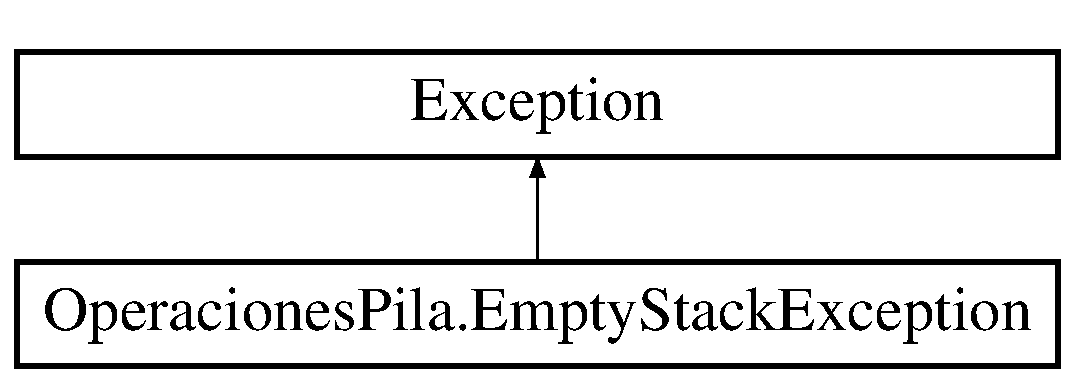
\includegraphics[height=2.000000cm]{class_operaciones_pila_1_1_empty_stack_exception}
\end{center}
\end{figure}
\subsection*{Public Member Functions}
\begin{DoxyCompactItemize}
\item 
\mbox{\Hypertarget{class_operaciones_pila_1_1_empty_stack_exception_a5336e29287c3a274358967d8ca2c22f9}\label{class_operaciones_pila_1_1_empty_stack_exception_a5336e29287c3a274358967d8ca2c22f9}} 
{\bfseries Empty\+Stack\+Exception} (string message)
\end{DoxyCompactItemize}


The documentation for this class was generated from the following file\+:\begin{DoxyCompactItemize}
\item 
D\+:/\+U\+N\+I/3er Semestre/\+Estructuras/\+S (3)/\+Operaciones\+Pila/\+Operaciones\+Pila/Empty\+Stack\+Exception.\+cs\end{DoxyCompactItemize}

\hypertarget{class_operaciones_pila_1_1_full_stack_exception}{}\section{Operaciones\+Pila.\+Full\+Stack\+Exception Class Reference}
\label{class_operaciones_pila_1_1_full_stack_exception}\index{Operaciones\+Pila.\+Full\+Stack\+Exception@{Operaciones\+Pila.\+Full\+Stack\+Exception}}
Inheritance diagram for Operaciones\+Pila.\+Full\+Stack\+Exception\+:\begin{figure}[H]
\begin{center}
\leavevmode
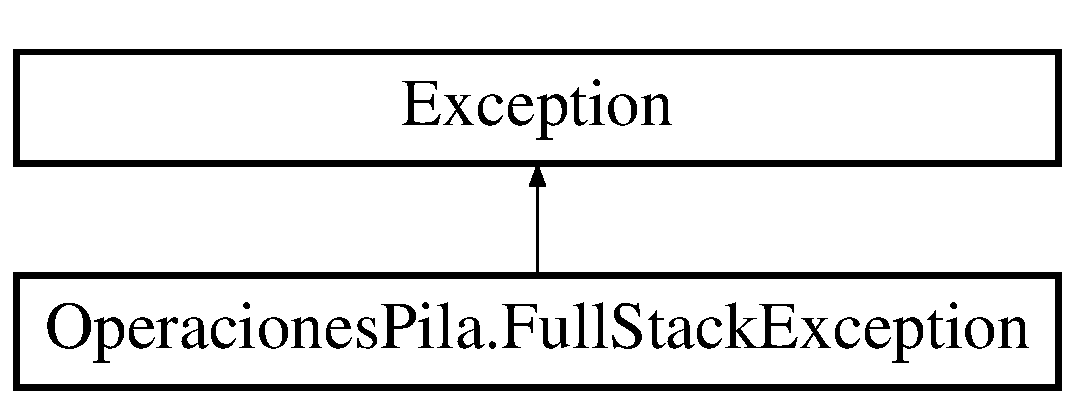
\includegraphics[height=2.000000cm]{class_operaciones_pila_1_1_full_stack_exception}
\end{center}
\end{figure}
\subsection*{Public Member Functions}
\begin{DoxyCompactItemize}
\item 
\mbox{\Hypertarget{class_operaciones_pila_1_1_full_stack_exception_a33d1e96f2e234cc2323a0409cedae4f7}\label{class_operaciones_pila_1_1_full_stack_exception_a33d1e96f2e234cc2323a0409cedae4f7}} 
{\bfseries Full\+Stack\+Exception} (string message)
\end{DoxyCompactItemize}


The documentation for this class was generated from the following file\+:\begin{DoxyCompactItemize}
\item 
D\+:/\+U\+N\+I/3er Semestre/\+Estructuras/\+S (3)/\+Operaciones\+Pila/\+Operaciones\+Pila/Full\+Stack\+Exception.\+cs\end{DoxyCompactItemize}

\hypertarget{class_operaciones_pila_1_1_main_window}{}\section{Operaciones\+Pila.\+Main\+Window Class Reference}
\label{class_operaciones_pila_1_1_main_window}\index{Operaciones\+Pila.\+Main\+Window@{Operaciones\+Pila.\+Main\+Window}}


Interaction logic for Main\+Window.\+xaml  


Inheritance diagram for Operaciones\+Pila.\+Main\+Window\+:\begin{figure}[H]
\begin{center}
\leavevmode
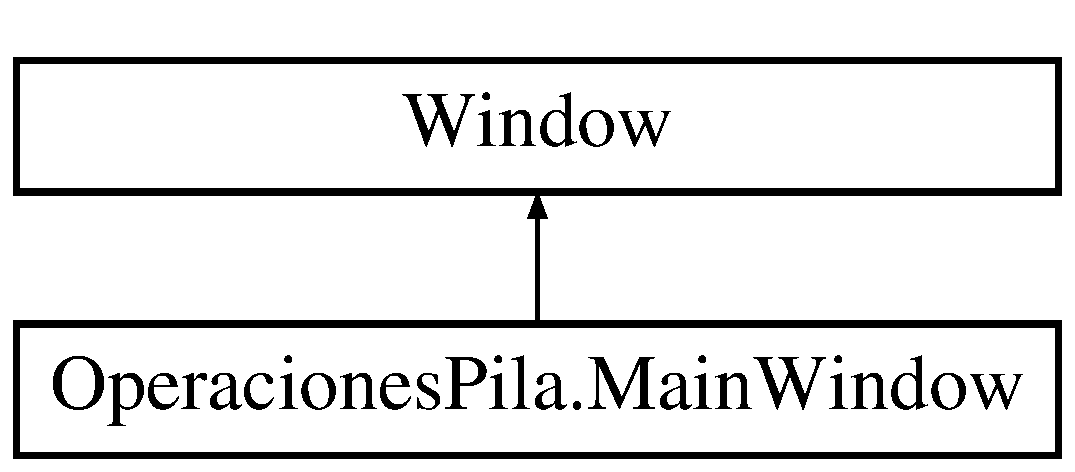
\includegraphics[height=2.000000cm]{class_operaciones_pila_1_1_main_window}
\end{center}
\end{figure}
\subsection*{Private Member Functions}
\begin{DoxyCompactItemize}
\item 
\mbox{\Hypertarget{class_operaciones_pila_1_1_main_window_af8d318be544f2f5b8f807724115b69e2}\label{class_operaciones_pila_1_1_main_window_af8d318be544f2f5b8f807724115b69e2}} 
void {\bfseries Window\+\_\+\+Loaded} (object sender, Routed\+Event\+Args e)
\item 
\mbox{\Hypertarget{class_operaciones_pila_1_1_main_window_af8d75db12c0004fd4cadbef9dd17db0f}\label{class_operaciones_pila_1_1_main_window_af8d75db12c0004fd4cadbef9dd17db0f}} 
void {\bfseries btn\+\_\+\+Push\+\_\+\+Click} (object sender, Routed\+Event\+Args e)
\item 
\mbox{\Hypertarget{class_operaciones_pila_1_1_main_window_a0977100f96e93631d8b42ee643af54c6}\label{class_operaciones_pila_1_1_main_window_a0977100f96e93631d8b42ee643af54c6}} 
void {\bfseries btn\+\_\+\+Pop\+\_\+\+Click} (object sender, Routed\+Event\+Args e)
\item 
\mbox{\Hypertarget{class_operaciones_pila_1_1_main_window_af21abb9c245d4c891b5fe7249b525ece}\label{class_operaciones_pila_1_1_main_window_af21abb9c245d4c891b5fe7249b525ece}} 
void {\bfseries btn\+\_\+\+Peek\+\_\+\+Click} (object sender, Routed\+Event\+Args e)
\end{DoxyCompactItemize}
\subsection*{Private Attributes}
\begin{DoxyCompactItemize}
\item 
\mbox{\Hypertarget{class_operaciones_pila_1_1_main_window_ac213011bd9e1929a3a7d586d243b5e37}\label{class_operaciones_pila_1_1_main_window_ac213011bd9e1929a3a7d586d243b5e37}} 
\hyperlink{class_operaciones_pila_1_1_array_stack}{Array\+Stack}$<$ string $>$ {\bfseries stack}
\end{DoxyCompactItemize}


\subsection{Detailed Description}
Interaction logic for Main\+Window.\+xaml 



The documentation for this class was generated from the following file\+:\begin{DoxyCompactItemize}
\item 
D\+:/\+U\+N\+I/3er Semestre/\+Estructuras/\+S (3)/\+Operaciones\+Pila/\+Operaciones\+Pila/Main\+Window.\+xaml.\+cs\end{DoxyCompactItemize}

%--- End generated contents ---

% Index
\backmatter
\newpage
\phantomsection
\clearemptydoublepage
\addcontentsline{toc}{chapter}{Index}
\printindex

\end{document}
